
% asset_id: FAS1VectorsTikZ-002
% asset_type: tikz
% topic_id: FAS1Vectors
% unit_code: FAS1
% topic_code: FAS1-VEC
% related_lesson_file: FAS1_vectors_lesson.md
% related_lesson_section: # 9. Visual Asset Integration
% source: FP1-Chp1-Vectors.pdf + transcripts.md where relevant
\documentclass[tikz,border=8pt]{standalone}
\usepackage{amsmath}
\usepackage{xcolor}
\usetikzlibrary{arrows.meta,calc,positioning}
\definecolor{Canvas}{HTML}{FAF9F6}
\definecolor{Ivory}{HTML}{FFFFF0}
\definecolor{LineGrey}{HTML}{E5E5EA}
\definecolor{Gold}{HTML}{C5A059}
\definecolor{TextInk}{HTML}{2C2C2E}
\definecolor{SoftPink}{HTML}{FBEFEF}
\begin{document}
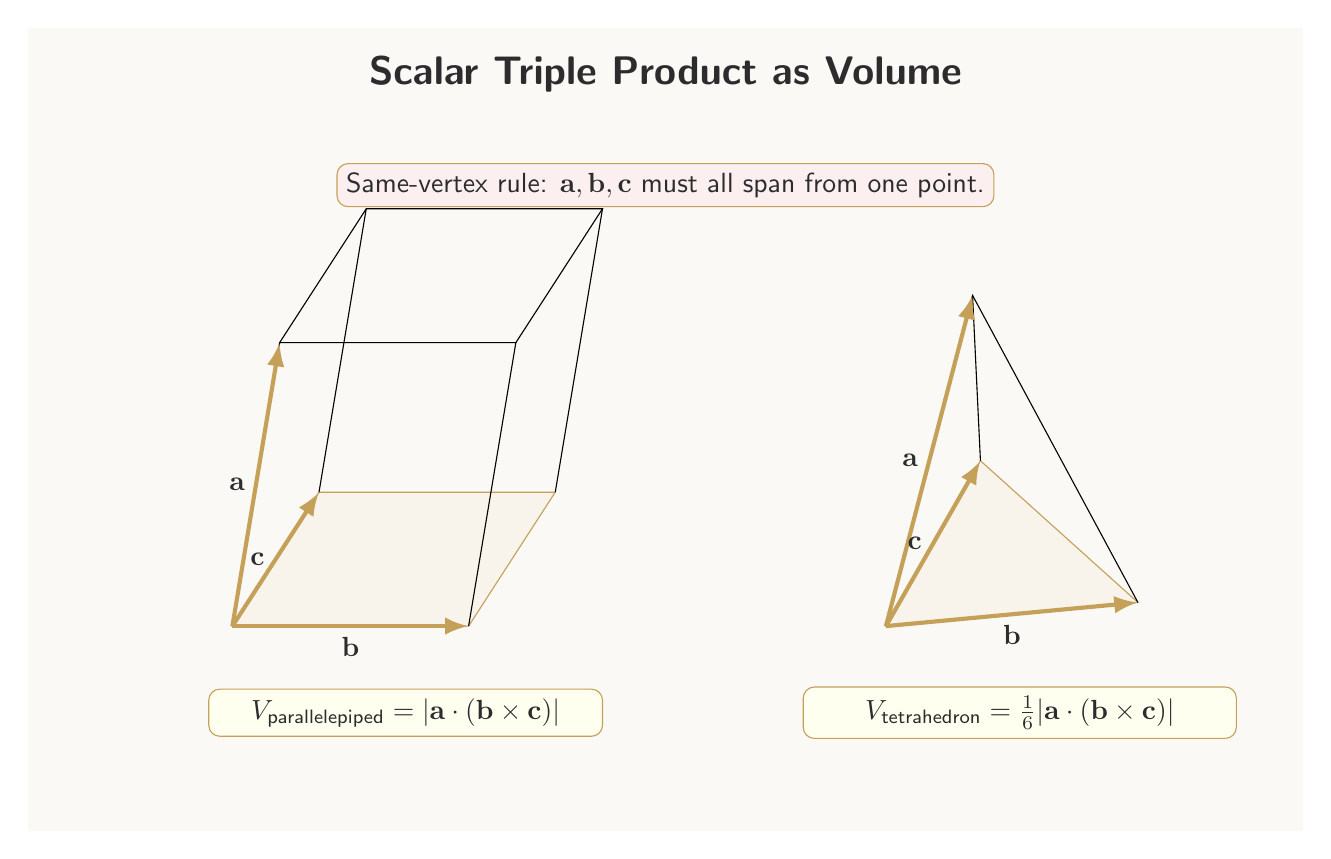
\begin{tikzpicture}[every node/.style={font=\sffamily,text=TextInk},arrow/.style={-{Latex[length=3mm]},line width=1.2pt,draw=TextInk},goldarrow/.style={-{Latex[length=3mm]},line width=1.5pt,draw=Gold}]
\fill[Canvas] (-0.6,-0.6) rectangle (15.6,9.6);

\node[font=\sffamily\bfseries\Large] at (7.5,9) {Scalar Triple Product as Volume};
\coordinate (O) at (2,2); \coordinate (B) at (5,2); \coordinate (C) at (3.1,3.7); \coordinate (A) at (2.6,5.6);
\coordinate (BC) at ($(B)+(C)-(O)$); \coordinate (BA) at ($(B)+(A)-(O)$); \coordinate (CA) at ($(C)+(A)-(O)$); \coordinate (BCA) at ($(B)+(C)+(A)-2*(O)$);
\filldraw[fill=Gold!12,draw=Gold] (O)--(B)--(BC)--(C)--cycle; \draw (O)--(A)--(BA)--(B); \draw (A)--(CA)--(BCA)--(BA); \draw (C)--(CA); \draw (BC)--(BCA);
\draw[goldarrow] (O)--(A) node[midway,left] {$\mathbf{a}$}; \draw[goldarrow] (O)--(B) node[midway,below] {$\mathbf{b}$}; \draw[goldarrow] (O)--(C) node[midway,left] {$\mathbf{c}$};
\node[draw=Gold,fill=Ivory,rounded corners,minimum width=5cm] at (4.2,0.9) {$V_{\text{parallelepiped}}=|\mathbf a\cdot(\mathbf b\times\mathbf c)|$};
\coordinate (T0) at (10.3,2); \coordinate (T1) at (13.5,2.3); \coordinate (T2) at (11.5,4.1); \coordinate (T3) at (11.4,6.2);
\filldraw[fill=Gold!12,draw=Gold] (T0)--(T1)--(T2)--cycle; \draw (T0)--(T3)--(T1); \draw (T2)--(T3);
\draw[goldarrow] (T0)--(T3) node[midway,left] {$\mathbf{a}$}; \draw[goldarrow] (T0)--(T1) node[midway,below] {$\mathbf{b}$}; \draw[goldarrow] (T0)--(T2) node[midway,left] {$\mathbf{c}$};
\node[draw=Gold,fill=Ivory,rounded corners,minimum width=5.5cm] at (12.0,0.9) {$V_{\text{tetrahedron}}=\frac16|\mathbf a\cdot(\mathbf b\times\mathbf c)|$};
\node[draw=Gold,fill=SoftPink,rounded corners] at (7.5,7.6) {Same-vertex rule: $\mathbf a,\mathbf b,\mathbf c$ must all span from one point.};

\end{tikzpicture}
\end{document}
